\documentclass[UTF8]{article}
\usepackage[UTF8]{ctex}
\usepackage[a4paper, margin=1in]{geometry}
\usepackage{amsmath}
\usepackage{subfigure}
% \usepackage{enumitem}
% \usepackage{ulem}
\usepackage{titlesec}
% \usepackage{CJKulem}
\usepackage{fancyhdr} % Required for custom headers
\usepackage{lastpage} % Required to determine the last page for the footer
\usepackage{graphicx} % Required to insert images


\cfoot{第\ \thepage\ 页}

\titlespacing*{\section} {1pt}{9pt}{0pt}
\titlespacing*{\subsection} {0pt}{3pt}{0pt}
% \setitemize[1]{itemsep=0pt,partopsep=0pt,parsep=\parskip,topsep=5pt}
\large
\title{Homework-Chapter 2}
\begin{document}

\begin{titlepage}
    \begin{center}
        \line(1,0){300}\\
        [0.65cm]
        \huge{\bfseries Assignment II }\\
        \line(1,0){300}\\
        \textsc{\Large Chapter IV}\\
        \textnormal{\Large \today}\\
        [5.5cm]
    \end{center}
    \begin{flushright}
        \texttt{\Large 谢远峰\\网安一班\\3019244283}\\
        [0.5cm]
    \end{flushright}
\end{titlepage}
\clearpage

\section*{Question1}
设置计时器是有必要的

- 往返延迟时间将使发送方知道数据包或数据包的ACK是否丢失。

- 计时器用于跟踪数据包的传输时间。

- 发送方需要一个计时器来检测每个数据包的丢失。
\section*{Question2}
\begin{figure}[ht]
    \centering  %图片全局居中
    \subfigure[New Packet]{
        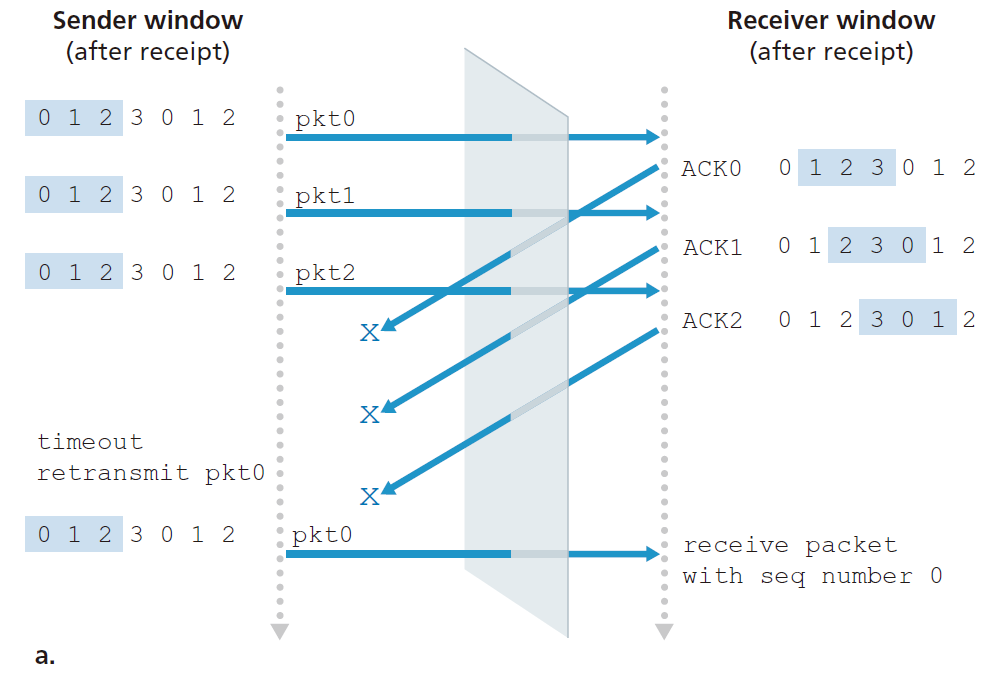
\includegraphics[width=0.45\textwidth]{2.png}}
    \subfigure[Retransmission]{
        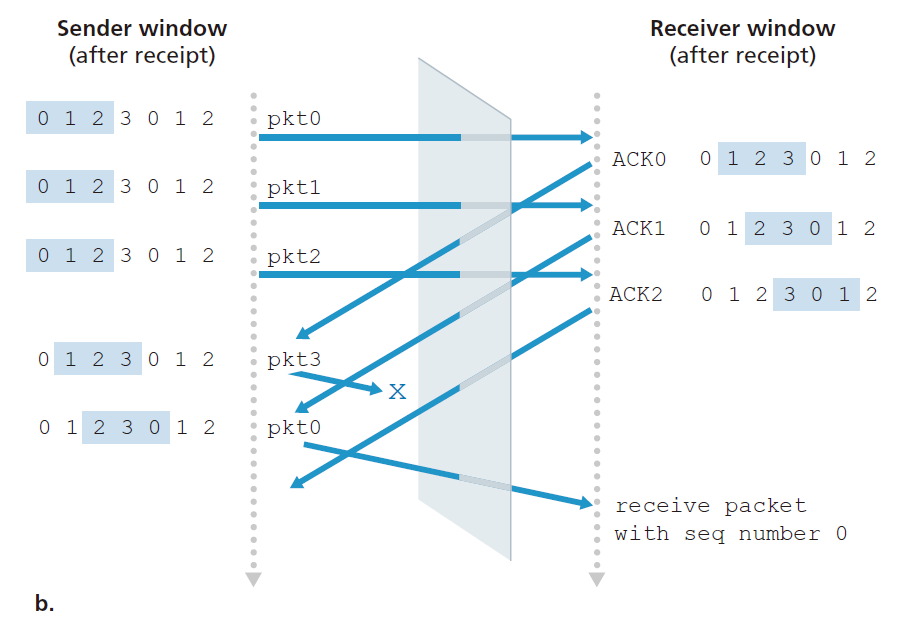
\includegraphics[width=0.45\textwidth]{4.png}}
    \caption{SR协议可能遇到的问题}
\end{figure}
发送方和接收方窗口间缺乏同步会产生严重的后果,有4个分组序列号且窗口长度为3,假定发送了分组0至2,并在接收方被正确接收且确认了。此时,接收方窗口落在第4、5、6个分组上,其序号分别为3、0、1。现在考虑两种情况。在第一种情况下,如a所示,对前3个分组的ACK丢失,因此发送方重传这些分组。因此,接收方下一步要接收序号为0的分组即第一个发送分组的副本。在第二种情况下,如b所示,对前3个分组的ACK都被正确交付。因此发送方向前移动窗口并发送第4、5、6个分组其序号分别为3、0、1。序号为3的分组丢失,但序号为0的分组到达(一个包含新数据的分组)。

考虑图中接收方的视角,在发送方和接收方之间有一个假想的帘子,因为接收方不能“看见”发送方采取的动作。接收方所能观察到的是它从信道中收到的以及它向信道中发出报文序列。就其所关注的而言,图中的两种情况是等同的。没有办法区分是第1个分组的重传还是第5个分组的初次传输。显然,窗口长度比序号空间小时协议无法工作。

为了避免出现图中显示的情况,需要避免接收方窗口的上界(接收方窗口的"最新"序列号)与发送方窗口下界(发送方窗口中 "最老"序列号)重叠。因此,序列号空间必须足够大,以适应整个接收方窗口和整个发送方窗口。

假设接收方正在等待的最低序列号是数据包m,在这种情况下,它的窗口[m, m+w-1],它已经接收数据包m-1(并发送ACK信息)和之前的w-1数据包,其中w是窗口的大小。如果这些w个ACK都还没有被发送者收到,那么数值为[m-w,m-1]的ACK信息可能还在传播回来。如果发送方没有收到这些ACK号码,那么发送方的窗口将是[m-w,m-1]。

因此,发送方窗口的下界是m-w,而接收方窗口的上界是m+w-1。为了使接收方窗口的上界不与发送方窗口的下界重叠,因此序列号长度至少为2w,以同时容纳发送方窗口大小+接收方窗口大小,即$w\leq k/2 $

\textmd{\textbf{SR协议发送方的窗口大小最大为$\left\lfloor k/2 \right\rfloor$}}

\section*{Question3}
\subsection*{a}
用$EstimatedRTT^{(n)}$表示对于第n个样例的预测
\begin{align*}
    EstimatedRTT^{(1)} & =  SampleRTT                                                           \\
    EstimatedRTT^{(2)} & = x * SampleRTT_{1}+(1-x) * SampleRTT_{2}                              \\
    EstimatedRTT^{(3)} & =   x * SampleRTT_{1}+(1-x)[x * SampleRTT_{2} +(1-x) * SampleRTT_{3}]  \\
                       & =
    x * SampleRTT_{1}+(1-x)x * SampleRTT_{2} +(1-x)^{2} * SampleRTT_{3}                         \\
    EstimatedRTT^{(4)} & =  x * SampleRTT_{1}+(1-x) * SampleRTT_{3}                             \\
                       & =  x * SampleRTT_{1}+(1-x)x * SampleRTT_{2}+(1-x)^{2}x * SampleRTT_{3} \\ & \quad+(1-x)^{3} * SampleRTT_{4} \\
\end{align*}
\vspace*{-1.5cm}
\subsection*{b}
$EstimatedRTT^{(n)} = x\sum\limits_{j=1}^{n-1}(1-x)^{j-1}*SampleRTT_{j}+(1-x)^{n-1}*SampleRTT_{n}$
\subsection*{c}
\vspace*{-1cm}
\begin{align*}
    EstimatedRTT^{\infty} & = \dfrac{\alpha}{1-\alpha}\sum\limits_{j= 1}^{\infty}(1-\alpha)^{j}*SampleRTT_{j} \\
                          & = \dfrac{1}{9}\sum\limits_{j=1}^{\infty}(0.9)^{j}*SampleRTT_{j}
\end{align*}

因为基于先前样本的权重以指数形式衰减,所以程序被称为指数移动平均。

\section*{Question4}
\subsection*{a}
\noindent
GBN:

A首先发送5个报文段(1,2,3,4,5),第二次重新发送4个报文段(2,3,4,5),总共发送9个报文段,A 发送的报文段顺序:1,2,3,4,5,2,3,4,5

B首先发送4个ACK(1,1,1,1),之后依次发送4个ACK(2,3,4,5),B 总共发送8个报文段,B 发送的ACK顺序:1,1,1,1,2,3,4,5

\noindent
SR:

A首先发送5个报文段(1,2,3,4,5),第二次重新发送1个报文段(2),总共发送6个报文段,A 发送的报文段顺序:1,2,3,4,5,2

B首先发送4个ACK(1,3,4,5),之后发送一个ACK(2),B 总共发送5个ACK,B 发送的ACK顺序:1,3,4,5,2

\noindent
TCP:

A首先发送5个报文段(1,2,3,4,5),第二次重新发送报文段(2),总共发送6个报文段,A 发送的报文段顺序:1,2,3,4,5,2

B首先发送4个ACK(2,2,2,2),之后发送ACK(6),B 总共发送5个ACK,B 发送的ACK顺序:2,2,2,2,6
\subsection*{b}
如果这三种协议的超时值都远长于5个RTT,由于TCP使用快速重传,不需要等待时间,所以能在最短的时间间隔内成功传送所有五个数据段。
\section*{Question5}
\begin{figure}[ht]
    \centering
    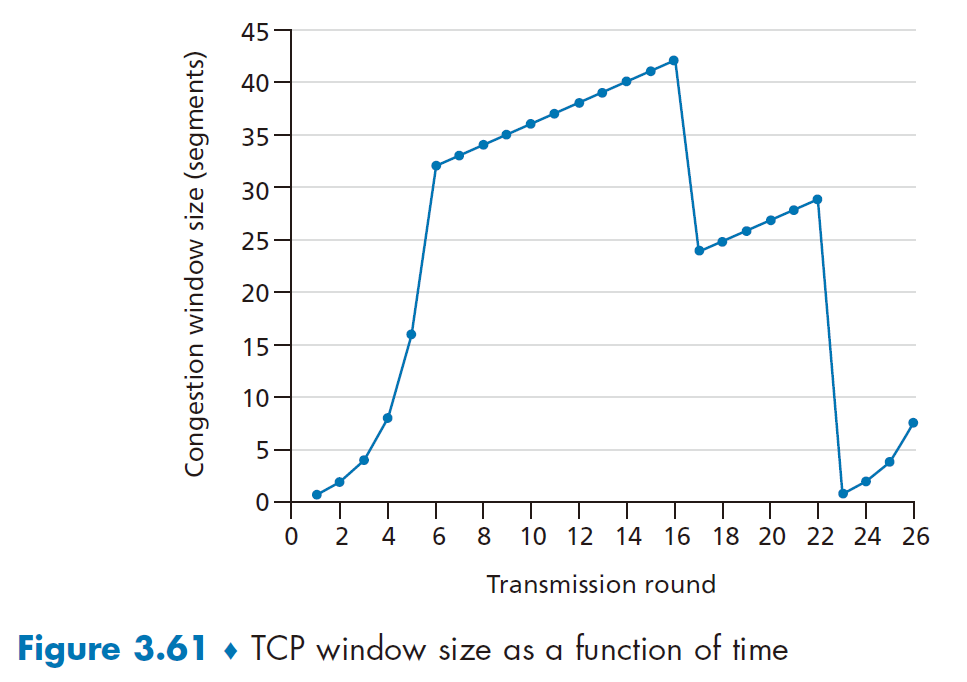
\includegraphics[width=10cm,height=6cm]{1.png}
\end{figure}
\subsection*{a}
\vspace*{-0.55cm}
TCP的慢启动区间在[1,6]和[23,26]
\subsection*{b}
\vspace*{-0.55cm}
TCP的拥塞避免区间在[6,16]和[17,22]
\subsection*{c}
\vspace*{-0.55cm}
由于重复接收到相同的ACK导致的丢包,如果为超时,发送窗口大小会降至1
\subsection*{d}
\vspace*{-0.55cm}
由于计时器超时导致的丢包,发送窗口大小降至1
\subsection*{e}
\vspace*{-0.55cm}
在第一个传输回合,慢启动阈值设置为32
\subsection*{f}
\vspace*{-0.55cm}
由于在第16个传输回合达到的窗口大小为42,检测到报文段的丢失,慢启动阈值减半,因此在第18个传输回合,慢启动阈值为21
\subsection*{g}
\vspace*{-0.55cm}
由于在第22个传输回合达到的窗口大小为29,计时器超时导致丢包事件出现,窗口大小归为1,进入慢启动阶段,因此在第23个传输回合,慢启动阈值为14
\subsection*{h}
\vspace*{-0.55cm}
第一传输回合,包1发送;第二个传输回合,包2-3发送;第三个传输回合,包4-7发送;第四个回合,包8-15发送;第五个回合,包16-31发送,第六个回合,包32-63发送;第七个回合,包64-96发送。因此,包70在第七个传输回合内发送
\subsection*{i}
\vspace*{-0.55cm}
第21个传输回合,检测到报文段丢失,当前拥塞窗口大小和慢启动阈值减半,设置为4,
\subsection*{j}
\vspace*{-0.55cm}
慢启动阈值为21,拥塞窗口大小为4
\subsection*{k}
\vspace*{-0.55cm}
传输回合17,1个包;传输回合18,2个包;传输回合19,4个包,传输回合20,8个包,传输回合21,16个包;传输回合22,21个包。因此总共用发送了52包
\end{document}